\chapter{Fundamentação Teórica} \label{cap:fundamentacao}

Este capítulo apresenta os conceitos que fundamentam o trabalho, organizados segundo as etapas do processo de descoberta de conhecimento em bases de dados, a mesma sequência adotada na metodologia.

Inicialmente, descrevem-se esse processo e suas etapas (Seção~\ref{sec:fund_kdd}). Em seguida, são abordados os conceitos associados a cada etapa: a compreensão e a exploração dos dados, incluindo o domínio clínico do problema (Seção~\ref{sec:fund_estatistica}); a preparação dos dados (Seção~\ref{sec:fund_preparacao}); os modelos de classificação utilizados (Seção~\ref{sec:fund_modelos}); o treinamento, a validação e a avaliação dos modelos (Seção~\ref{sec:fund_validacao}); e a interpretação dos modelos (Seção~\ref{sec:fund_interpretabilidade}). Por fim, discute-se o viés algorítmico em saúde (Seção~\ref{sec:fund_vies}). Os termos básicos de estatística e aprendizado de máquina estão reunidos no Glossário (página~\pageref{glossario}), e os símbolos matemáticos, na Lista de Símbolos.

\section{Mineração de Dados e Descoberta de Conhecimento}
\label{sec:fund_kdd}

A descoberta de conhecimento em bases de dados (\textit{Knowledge Discovery in Databases}, KDD) é o processo de identificação de padrões válidos, novos e potencialmente úteis em conjuntos de dados \cite{Fayyad1996KDD}. A mineração de dados corresponde à etapa em que algoritmos extraem esses padrões; o resultado, entretanto, depende também da preparação dos dados que a antecede e da interpretação que a sucede, e o processo é iterativo \cite{Fayyad1996KDD}.

Neste trabalho, o processo foi organizado em cinco etapas (Figura~\ref{fig:fund_kdd}), cuja implementação computacional é denominada \textit{pipeline}. Na compreensão e exploração, caracterizam-se o problema e os dados; na preparação, os dados são tratados e transformados; na modelagem, os algoritmos são ajustados aos dados; no treinamento, validação e avaliação, estima-se o desempenho dos modelos; e, na interpretação, analisa-se de que forma os modelos produzem suas previsões. As setas tracejadas indicam que o processo não é linear, podendo um resultado de avaliação motivar a revisão de etapas anteriores. A ordem das operações foi definida de modo a evitar o vazamento de dados (Seção~\ref{sec:fund_vazamento}) \cite{KaufmanScharRosset2012, KAPOOR2023100804}.

Como diversas etapas envolvem procedimentos aleatórios, como a divisão entre treino e teste, a validação cruzada e o SMOTE, fixa-se a semente aleatória, isto é, o valor inicial do gerador de números pseudoaleatórios. A fixação da semente garante que os mesmos sorteios sejam reproduzidos em cada execução e, consequentemente, a reprodutibilidade dos resultados \cite{Pineau2020Improving}.

\begin{figure}[htbp]
\centering
\begin{tikzpicture}[
    etapa/.style={rectangle, rounded corners, draw, thick, align=center, text width=2.65cm, minimum height=1.8cm, font=\footnotesize\bfseries},
    itens/.style={rectangle, draw, align=left, text width=2.65cm, minimum height=2.7cm, font=\scriptsize, inner sep=3pt},
    seta/.style={->, thick, >=stealth}]
\node[etapa] (a) {1. Compreensão e exploração};
\node[etapa, right=0.3cm of a] (b) {2. Preparação dos dados};
\node[etapa, right=0.3cm of b] (c) {3. Modelagem};
\node[etapa, right=0.3cm of c] (d) {4. Treinamento, validação e avaliação};
\node[etapa, right=0.3cm of d] (e) {5. Interpretação dos modelos};
\node[itens, below=0.15cm of a, anchor=north] {\textbullet~Caracterização e qualidade da base\\ \textbullet~Estatísticas e assimetria\\ \textbullet~Comparação entre classes\\ \textbullet~Correlação};
\node[itens, below=0.15cm of b, anchor=north] {\textbullet~Remoção de duplicatas\\ \textbullet~Transformação logarítmica\\ \textbullet~Divisão treino/teste\\ \textbullet~Imputação\\ \textbullet~Padronização\\ \textbullet~SMOTE (só no treino)};
\node[itens, below=0.15cm of c, anchor=north] {\textbullet~Regressão Logística\\ \textbullet~\textit{Random Forest}\\ \textbullet~XGBoost\\ \textbullet~LightGBM};
\node[itens, below=0.15cm of d, anchor=north] {\textbullet~Validação cruzada repetida\\ \textbullet~Busca aleatória de hiperparâmetros\\ \textbullet~Seleção pela AUC-ROC\\ \textbullet~Avaliação no teste e limiares\\ \textbullet~Comparação entre modelos};
\node[itens, below=0.15cm of e, anchor=north] {\textbullet~SHAP (TreeSHAP e Monte Carlo)\\ \textbullet~Importância global e local\\ \textbullet~Auditoria por sexo\\ \textbullet~Comparação de rankings};
\draw[seta] (a) -- (b);
\draw[seta] (b) -- (c);
\draw[seta] (c) -- (d);
\draw[seta] (d) -- (e);
\draw[seta, dashed] (d.north) -- ++(0,0.6) -| node[pos=0.25, above, font=\footnotesize] {retorno às etapas anteriores, quando necessário} (a.north);
\end{tikzpicture}

\caption{Fluxo (\textit{pipeline}) adotado neste trabalho, organizado nas etapas do processo de descoberta de conhecimento.}
\label{fig:fund_kdd}
{\small Fonte: elaborado pelo autor, com base em \citeonline{Fayyad1996KDD}.}
\end{figure}

A Tabela~\ref{tab:fund_kdd} apresenta a correspondência entre cada etapa do processo e os procedimentos realizados neste trabalho, detalhados no Capítulo~\ref{metodologia}.

\begin{table}[htbp]
\centering
\begin{tabular}{>{\raggedright\arraybackslash}p{4.2cm}>{\raggedright\arraybackslash}p{9.8cm}}
\hline
\textbf{Etapa} & \textbf{Procedimentos realizados} \\
\hline
Compreensão e exploração dos dados & Escolha da base ILPD; verificação de qualidade, valores ausentes e duplicatas; estatísticas descritivas, assimetria, comparação entre doentes e saudáveis e correlação entre os exames. \\[0.1cm]
Preparação dos dados & Remoção de duplicatas; transformação logarítmica dos exames assimétricos; divisão em treino e teste; imputação pela mediana; padronização; balanceamento com SMOTE apenas no treino. \\[0.1cm]
Modelagem & Treinamento da Regressão Logística, do \textit{Random Forest}, do XGBoost e do LightGBM. \\[0.1cm]
Treinamento, validação e avaliação & Validação cruzada repetida; busca aleatória de hiperparâmetros; avaliação no conjunto de teste com matriz de confusão, AUC e teste de DeLong; limiar clínico; avaliação por sexo. \\[0.1cm]
Interpretação dos modelos & Valores SHAP: importância das variáveis, sentido e forma dos efeitos, explicação de pacientes individuais, auditoria por sexo e comparação entre modelos. \\
\hline
\end{tabular}
\caption{Correspondência entre as etapas do processo de descoberta de conhecimento e os procedimentos deste trabalho.}
\label{tab:fund_kdd}
\par\vspace{2pt}{\small Fonte: elaborado pelo autor.}
\end{table}

\section{Compreensão e Exploração dos Dados}
\label{sec:fund_estatistica}

A Análise Exploratória de Dados (AED) reúne resumos numéricos e representações gráficas empregados para caracterizar a estrutura e a qualidade das variáveis antes da modelagem \cite{exploratorydataanalysis}. Nessa etapa, identificam-se valores ausentes, registros duplicados, valores extremos e variáveis redundantes, achados que orientam as decisões de preparação dos dados. A AED tem caráter exclusivamente descritivo: nenhuma estatística nela calculada deve ser utilizada para transformar os dados empregados no ajuste dos modelos (Seção~\ref{sec:fund_vazamento}).

\subsection{Domínio do Problema: Doença Hepática e Marcadores Laboratoriais}
\label{sec:fund_figado}

O fígado é responsável pela síntese da maior parte das proteínas plasmáticas, como a albumina, e pela eliminação da bilirrubina, pigmento resultante da degradação da hemoglobina. Doença hepática é o termo geral que designa as condições que lesam o fígado ou comprometem seu funcionamento, como as hepatites e a cirrose. Sua investigação inicial recorre a exames laboratoriais, cujos valores podem atingir várias vezes o limite superior da faixa de referência \cite{Giannini2005Liver, Kwo2016ACG}.

Cada marcador reflete um aspecto da função hepática. A alanina aminotransferase (ALT) e a aspartato aminotransferase (AST) são enzimas intracelulares liberadas na circulação quando há lesão dos hepatócitos e, por isso, tendem a elevar-se conjuntamente \cite{Kwo2016ACG, Newsome2018Guidelines}. A fosfatase alcalina eleva-se na obstrução do fluxo biliar, e a bilirrubina, em ambas as situações; a bilirrubina direta corresponde à fração conjugada pelo fígado e integra a bilirrubina total \cite{Kwo2016ACG}. As proteínas totais, a albumina e a razão albumina/globulina refletem a capacidade de síntese proteica, e a redução da albumina indica comprometimento dessa função \cite{Busher1990Albumin}. Em consequência, diversos exames carregam informação parcialmente redundante e são correlacionados, e suas distribuições são assimétricas, com valores extremos que decorrem da própria doença, e não necessariamente de erros de medição.

\subsection{Conceitos Básicos de Dados e Aprendizado Supervisionado}
\label{sec:fund_conceitos}

Em uma base de dados tabular, cada linha corresponde a uma observação, neste trabalho um paciente, e cada coluna, a uma variável. As variáveis podem ser numéricas, como os exames laboratoriais, ou categóricas, como o sexo. No aprendizado supervisionado, uma das variáveis é a variável-alvo, que se deseja prever, e as demais são os preditores; quando a variável-alvo é categórica, a tarefa é denominada classificação \cite{elementsofstatiscal}. O modelo é ajustado em um conjunto de treino e avaliado em um conjunto de teste, independente, que representa observações não vistas durante o ajuste \cite{elementsofstatiscal}.

Em problemas com duas classes, denomina-se positiva a classe que se deseja detectar, neste trabalho ``doente'', e negativa a outra, ``saudável''. A base é dita desbalanceada quando uma das classes, a majoritária, possui número de observações substancialmente maior que a outra, a minoritária. A proporção de observações de uma classe é denominada prevalência.

\subsection{Estatísticas Descritivas e Assimetria}
\label{sec:fund_assimetria}

As estatísticas descritivas resumem a distribuição de uma variável. A média é sensível a valores extremos (\textit{outliers}), ao passo que a mediana é pouco afetada por eles \cite{han2012getting}; assim, uma média consideravelmente superior à mediana indica a presença de uma cauda de valores elevados, isto é, de assimetria positiva.

O coeficiente de assimetria (\textit{skewness}) quantifica esse comportamento: assume valores próximos de zero em distribuições simétricas e valores positivos quando poucos valores muito elevados formam uma cauda à direita, situação frequente em exames laboratoriais. A assimetria acentuada distorce estatísticas como a média e o coeficiente de correlação de Pearson e confere peso excessivo a poucas observações em modelos lineares, como a Regressão Logística. Não há um limite universal para caracterizar a assimetria como excessiva; \citeonline[p.~26]{curran1996robustness} identificaram problemas a partir de 2,0, valor adotado neste trabalho como convenção. No contexto da doença hepática, valores extremos podem constituir o próprio fenômeno de interesse e, portanto, não devem ser descartados \cite[p.~237]{Aggarwal2015}.

\subsection{Correlação e Multicolinearidade}
\label{sec:fund_correlacao}

O coeficiente de correlação de Pearson ($r$) mede o grau de associação linear entre duas variáveis e varia de $-1$ a $+1$; valores próximos de zero indicam ausência de associação linear, e valores absolutos superiores a 0,7 costumam indicar correlação forte \cite{Dormann2013Collinearity}. O coeficiente de correlação de Spearman é calculado sobre os postos, isto é, sobre as posições dos valores ordenados, e é menos sensível a valores extremos \cite{Schober2018Correlation}.

Quando preditores são fortemente correlacionados entre si, ocorre multicolinearidade: as variáveis carregam informação semelhante, o que afeta principalmente a interpretação dos modelos, e não sua capacidade preditiva \cite{Strobl2008Conditional, Dormann2013Collinearity}. É o que ocorre com as bilirrubinas total e direta, cuja variação conjunta impede que o modelo atribua a cada uma, isoladamente, sua contribuição para a previsão.

\subsection{Testes de Hipótese e Comparações Múltiplas}
\label{sec:fund_bonferroni}

Um teste de hipótese avalia se os dados fornecem evidência contra uma hipótese nula, que em geral estabelece a ausência de diferença ou de efeito. O valor-$p$ corresponde à probabilidade de se observar um resultado ao menos tão extremo quanto o obtido, supondo verdadeira a hipótese nula. Rejeita-se a hipótese nula quando o valor-$p$ é inferior ao nível de significância adotado, convencionalmente 0,05. Neste trabalho, testes de hipótese são empregados na avaliação dos coeficientes da Regressão Logística e na comparação do desempenho dos modelos.

Quando diversos testes são realizados sobre os mesmos dados, aumenta a probabilidade de que algum resultado seja considerado significativo apenas por acaso. A correção de Bonferroni controla esse efeito multiplicando cada valor-$p$ pelo número de comparações realizadas, com limite superior igual a 1 \cite{Demsar2006Statistical}. Trata-se de uma correção conservadora, que reduz a ocorrência de falsos positivos à custa de menor capacidade de detectar diferenças reais.

\section{Preparação dos Dados}
\label{sec:fund_preparacao}

A preparação dos dados converte os dados brutos em uma representação adequada aos algoritmos e pode influenciar o resultado tanto quanto a escolha do modelo \cite{KAPOOR2023100804}. Ela compreende o tratamento de valores ausentes e de registros duplicados, a transformação da escala das variáveis e o balanceamento das classes, sempre de modo a impedir que informação do conjunto de teste seja utilizada no treinamento.

\subsection{Valores Ausentes, Registros Duplicados e Vazamento de Dados}
\label{sec:fund_ausentes}
\label{sec:fund_vazamento}

Valores ausentes correspondem a informações não registradas para algumas observações. Em vez da exclusão das observações afetadas, pode-se recorrer à imputação, que substitui cada valor ausente por uma estimativa; a mediana é preferível à média por ser robusta aos valores extremos característicos dos exames laboratoriais \cite{batistamonard2003}. Registros duplicados, por sua vez, são observações idênticas em todas as variáveis.

Ambos os casos relacionam-se ao vazamento de dados (\textit{data leakage}), que ocorre quando informação do conjunto de teste é incorporada, direta ou indiretamente, ao treinamento, o que torna a estimativa de desempenho excessivamente otimista \cite{KaufmanScharRosset2012, KAPOOR2023100804}. O vazamento pode decorrer da presença de um registro no treino e de sua duplicata no teste, do cálculo de parâmetros de transformação, como a mediana da imputação ou a média da padronização, a partir de todos os dados, ou do balanceamento das classes antes da divisão (Seção~\ref{sec:fund_smote}). Por esse motivo, tais operações devem ser ajustadas exclusivamente no conjunto de treino e, em seguida, aplicadas ao conjunto de teste.

\subsection{Transformação Logarítmica e Padronização}
\label{sec:fund_log}
\label{sec:fund_padronizacao}

Variáveis com distribuição de cauda longa, como os exames hepáticos, podem ter sua assimetria reduzida por meio da transformação logarítmica \cite{logtransformation}:
\begin{equation}
    x' = \ln(1 + x),
    \label{eq:log}
\end{equation}
em que $x$ é o valor original e $x'$, o valor transformado. A transformação comprime proporcionalmente mais os valores elevados do que os reduzidos, preservando a ordem entre as observações. No ILPD, a AST apresenta mediana de 42~IU/L e máximo de 4.929~IU/L; após a transformação, esses valores passam a 3,76 e 8,50, respectivamente. A adição de uma unidade evita a indefinição do logaritmo para valores nulos. Como a transformação nem sempre reduz a assimetria, seu efeito deve ser verificado pelo recálculo do coeficiente de assimetria \cite{logtransformation}. Por depender apenas do valor de cada observação, e não de parâmetros estimados a partir dos dados, a transformação pode ser aplicada antes da divisão entre treino e teste sem ocasionar vazamento.

A padronização (\textit{z-score}), definida por $z = (x - \bar{x})/s$, expressa cada valor em número de desvios-padrão em relação à média, de modo que todas as variáveis passam a ter média zero e desvio-padrão unitário. Como a média $\bar{x}$ e o desvio-padrão $s$ são estimados a partir dos dados, devem ser calculados apenas no conjunto de treino e, posteriormente, aplicados ao conjunto de teste.

Ambas as operações são relevantes principalmente para a Regressão Logística: a padronização torna os coeficientes comparáveis entre si, pois cada um passa a expressar o efeito de um desvio-padrão \cite{Hosmer2005Applied}, e a transformação logarítmica reduz a influência das observações extremas sobre o ajuste. Para os modelos baseados em árvores de decisão, o efeito é reduzido, uma vez que as divisões dependem apenas da ordem dos valores, preservada por transformações monotônicas \cite{elementsofstatiscal}.

\subsection{Desbalanceamento de Classes e SMOTE}
\label{sec:fund_smote}

Em bases desbalanceadas, um classificador pode obter acurácia elevada prevendo sempre a classe majoritária \cite{FAWCETT2006861}. No ILPD, em que 71\% dos pacientes pertencem à classe ``doente'', esse classificador trivial apresentaria acurácia de 71\% sem identificar nenhum paciente saudável.

O SMOTE (\textit{Synthetic Minority Over-sampling Technique}) \cite{smote} é uma técnica de sobreamostragem que gera observações sintéticas da classe minoritária. Para cada observação dessa classe, seleciona-se aleatoriamente um de seus $k$ vizinhos mais próximos da mesma classe, e a nova observação é gerada em um ponto sorteado do segmento que une as duas. Em variáveis binárias, como o sexo, essa interpolação produz valores sem significado, limitação tratada pela variante SMOTE-NC \cite{smote}.

A reamostragem deve ser aplicada exclusivamente ao conjunto de treino e, quando há validação cruzada, dentro de cada partição de treino, a fim de evitar vazamento \cite{KaufmanScharRosset2012}. Além disso, ao alterar a proporção de classes apresentada ao modelo, o SMOTE faz com que as probabilidades previstas deixem de refletir a prevalência real \cite{vandenGoorbergh2022Harm}, tendendo, neste caso, a subestimar a probabilidade de doença.

\section{Modelagem e Classificação}
\label{sec:fund_modelos}

Um modelo de classificação recebe os preditores de uma observação e estima a probabilidade de que ela pertença à classe positiva. O principal risco do treinamento é o sobreajuste (\textit{overfitting}), situação em que o modelo se ajusta a particularidades e ruídos do conjunto de treino e apresenta baixa capacidade de generalização para novas observações.

Neste trabalho, foram empregados quatro modelos: a Regressão Logística e três métodos de \textit{ensemble} baseados em árvores de decisão. A inclusão da Regressão Logística como referência fundamenta-se na revisão sistemática de \citeonline{Christodoulou2019Systematic}, que, ao analisar 71 estudos de predição clínica, não identificou vantagem dos métodos de aprendizado de máquina sobre a regressão logística nas comparações com baixo risco de viés.

\subsection{Regressão Logística}
\label{sec:fund_lr}

A Regressão Logística \cite{Cox1958Regression} modela o logaritmo da chance (\textit{odds}), definida como a razão entre a probabilidade de ocorrência do evento e a de sua não ocorrência, como uma combinação linear dos preditores \cite{Hosmer2005Applied}:
\begin{equation}
    \ln\left(\frac{\pi(\mathbf{x})}{1 - \pi(\mathbf{x})}\right) = \beta_0 + \sum_{j=1}^{p} \beta_j x_j,
    \label{eq:logit}
\end{equation}
em que $\pi(\mathbf{x})$ é a probabilidade de doença, $\beta_0$ é o intercepto e $\beta_j$ é o coeficiente associado ao preditor $x_j$. A significância de cada coeficiente é avaliada pelo teste de Wald.

A principal vantagem do modelo é a interpretação direta de seus coeficientes: mantidos constantes os demais preditores, o aumento de uma unidade em $x_j$ multiplica a chance de doença pela razão de chances $e^{\beta_j}$ \cite{Hosmer2005Applied}. Essa interpretação torna-se pouco confiável na presença de preditores fortemente correlacionados, cujos coeficientes são instáveis e podem inclusive apresentar sinal oposto ao esperado \cite{Dormann2013Collinearity}.

\subsection{Árvores de Decisão e Métodos de \textit{Ensemble}}
\label{sec:fund_arvores}

Uma árvore de decisão classifica uma observação por meio de uma sequência de regras sobre as variáveis, organizadas hierarquicamente, até alcançar um nó terminal, denominado folha, que indica a classe prevista \cite{elementsofstatiscal}. A Figura~\ref{fig:fund_arvore} apresenta um exemplo ilustrativo. Árvores individuais são de fácil interpretação, mas instáveis: pequenas alterações no conjunto de treino podem produzir árvores substancialmente diferentes.

Os métodos de \textit{ensemble} combinam múltiplas árvores para reduzir essa instabilidade. No \textit{bagging}, as árvores são treinadas de forma independente, cada uma em uma amostra distinta dos dados, e suas previsões são combinadas por votação. No \textit{boosting}, as árvores são treinadas sequencialmente, cada uma buscando corrigir os erros das anteriores. Em contrapartida, o modelo resultante perde a interpretabilidade direta e passa a ser considerado um modelo de caixa-preta.

\begin{figure}[htbp]
\centering
\begin{tikzpicture}[
    perg/.style={rectangle, rounded corners, draw, thick, align=center, font=\footnotesize, inner sep=4pt},
    folha/.style={rectangle, draw, fill=gray!20, align=center, font=\footnotesize, inner sep=4pt},
    level distance=1.6cm, sibling distance=5.2cm, edge from parent/.style={draw, -{Stealth}, thick}]
\node[perg] {Bilirrubina total $> 1{,}8$~mg/dL?}
  child {node[folha] {Doente}
    edge from parent node[left, font=\scriptsize, xshift=-3pt] {sim}}
  child {node[perg] {AST $> 60$~IU/L?}
    child {node[folha] {Doente} edge from parent node[left, font=\scriptsize, xshift=-3pt] {sim}}
    child {node[folha] {Saudável} edge from parent node[right, font=\scriptsize, xshift=3pt] {não}}
    edge from parent node[right, font=\scriptsize, xshift=3pt] {não}};
\end{tikzpicture}
\caption{Exemplo ilustrativo de árvore de decisão com dois exames do ILPD. Os pontos de corte são apenas ilustrativos.}
\label{fig:fund_arvore}
{\small Fonte: elaborado pelo autor.}
\end{figure}

\subsection{\textit{Random Forest}}
\label{sec:fund_rf}

O \textit{Random Forest} \cite{Breiman2001RandomForests} aplica o \textit{bagging} a árvores de decisão. Cada árvore é treinada em uma amostra \textit{bootstrap}, obtida por sorteio com reposição a partir do conjunto de treino, e, em cada divisão, apenas um subconjunto aleatório de \texttt{mtry} variáveis é considerado, o que aumenta a diversidade entre as árvores. A probabilidade estimada de doença corresponde à fração de árvores que atribuem a observação a essa classe. O aumento do número de árvores não provoca sobreajuste, e o método tende a apresentar bom desempenho com os valores padrão de seus hiperparâmetros \cite{Breiman2001RandomForests, Probst2019Hyperparameters}.

\subsection{XGBoost}
\label{sec:fund_xgb}

O XGBoost \cite{Chen2016XGBoost} é uma implementação regularizada do \textit{gradient boosting} \cite{Friedman2001Greedy}, método em que cada nova árvore é ajustada aos resíduos das previsões acumuladas até a iteração anterior. A previsão final é a soma das contribuições de todas as árvores, convertida em probabilidade pela função logística:
\begin{equation}
    F(\mathbf{x}) = \sum_{m=1}^{M} f_m(\mathbf{x}),
    \qquad
    \hat{\pi}(\mathbf{x}) = \frac{1}{1 + e^{-F(\mathbf{x})}},
    \label{eq:boosting}
\end{equation}
em que $f_m$ é a $m$-ésima árvore, $M$ é o número de iterações e $F(\mathbf{x})$ é expresso na escala do logaritmo da chance.

Para controlar o sobreajuste, a taxa de aprendizado $\eta$ reduz a contribuição de cada árvore, e os termos de regularização $\gamma$ e $\lambda$ penalizam, respectivamente, o número de folhas e a magnitude dos valores atribuídos a elas \cite{Chen2016XGBoost}. Em dados tabulares, o XGBoost figura entre os métodos de melhor desempenho \cite{Grinsztajn2022Why}.

\subsection{LightGBM}
\label{sec:fund_lgbm}

O LightGBM \cite{Ke2017LightGBM} baseia-se no mesmo princípio de \textit{boosting} (Equação~\ref{eq:boosting}), com ênfase na eficiência computacional. O algoritmo discretiza os valores contínuos em intervalos e expande cada árvore a partir da folha que proporciona maior redução do erro (\textit{leaf-wise}), em vez de expandi-la nível a nível. Em bases pequenas, essa estratégia pode favorecer o sobreajuste, razão pela qual se recomenda limitar o número de folhas e estabelecer um número mínimo de observações por folha \cite{LightGBMDocsTuning}.

\section{Treinamento, Validação e Avaliação}
\label{sec:fund_validacao}

Além do ajuste aos dados de treino, é necessário estimar o desempenho do modelo em observações não utilizadas no treinamento, isto é, sua capacidade de generalização. Esta seção trata da estimação do desempenho sem o uso do conjunto de teste, da escolha das configurações dos algoritmos, das métricas de avaliação e da definição do limiar de decisão.

\subsection{Validação Cruzada}
\label{sec:fund_cv}

Na validação cruzada $k$-\textit{fold}, o conjunto de treino é dividido em $k$ partes de tamanhos semelhantes, denominadas \textit{folds}. O modelo é treinado com $k-1$ partes e avaliado na parte restante, procedimento repetido até que cada parte tenha sido utilizada uma vez para avaliação (Figura~\ref{fig:fund_cv}). O desempenho estimado corresponde à média das $k$ avaliações \cite{elementsofstatiscal}.

\begin{figure}[htbp]
\centering
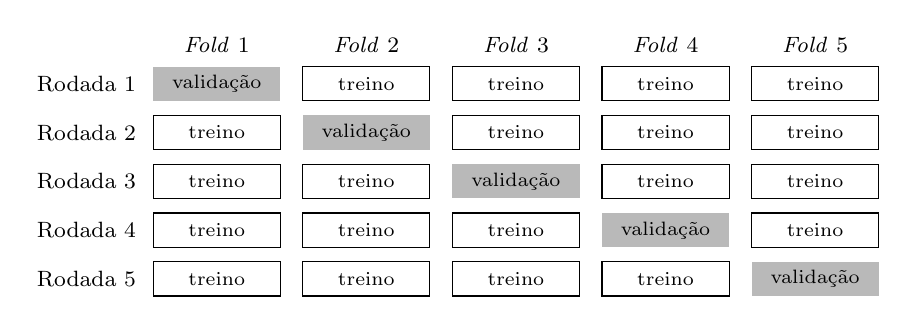
\begin{tikzpicture}[x=1.9cm, y=0.62cm]
\foreach \lin in {1,...,5} {
  \node[anchor=east, font=\footnotesize] at (0.05,-\lin) {Rodada \lin};
  \foreach \col in {1,...,5} {
    \ifnum\col=\lin
      \fill[gray!55] (\col-1+0.1,-\lin-0.35) rectangle (\col-0.05,-\lin+0.35);
      \node[font=\scriptsize] at (\col-0.475,-\lin) {validação};
    \else
      \draw (\col-1+0.1,-\lin-0.35) rectangle (\col-0.05,-\lin+0.35);
      \node[font=\scriptsize] at (\col-0.475,-\lin) {treino};
    \fi
  }
}
\foreach \col in {1,...,5} { \node[font=\footnotesize] at (\col-0.475,-0.2) {\textit{Fold} \col}; }
\end{tikzpicture}
\caption{Validação cruzada com $k = 5$: em cada rodada, uma parte diferente do conjunto de treino é usada para avaliar o modelo treinado com as outras quatro.}
\label{fig:fund_cv}
{\small Fonte: elaborado pelo autor.}
\end{figure}

As previsões obtidas para as observações da parte reservada, produzidas por um modelo que não as utilizou no ajuste, são denominadas previsões fora da partição (\textit{out-of-fold}). Ao final das $k$ rodadas, cada observação do treino dispõe de uma previsão desse tipo, o que permite, entre outras aplicações, a escolha do limiar de decisão sem o uso do conjunto de teste (Seção~\ref{sec:fund_limiar}). A estratificação preserva, em cada parte, a proporção de classes da base. Os valores mais utilizados de $k$ são 5 e 10, que representam um compromisso entre o viés e a variância da estimativa \cite{elementsofstatiscal}. Como o resultado depende da alocação das observações entre as partes, o procedimento pode ser repetido com diferentes sorteios, o que reduz a variabilidade da estimativa \cite{Kim2009Estimating}.

\subsection{Hiperparâmetros e Sua Otimização}
\label{sec:fund_hiperparametros}

Os parâmetros de um modelo são estimados a partir dos dados durante o treinamento, como os coeficientes da Regressão Logística. Os hiperparâmetros, por sua vez, são definidos antes do treinamento e controlam o processo de aprendizado, como o número de variáveis consideradas em cada divisão do \textit{Random Forest}, a profundidade máxima das árvores e a taxa de aprendizado do XGBoost.

A otimização de hiperparâmetros consiste em avaliar diferentes combinações, em geral por validação cruzada, e selecionar a de melhor desempenho. Na busca em grade, avaliam-se todas as combinações de um conjunto predefinido de valores, cujo número cresce exponencialmente com a quantidade de hiperparâmetros. Na busca aleatória, avalia-se um número fixo de combinações sorteadas, estratégia que tende a obter resultados comparáveis aos da busca em grade com custo computacional muito inferior \cite{Bergstra2012Random}. Como a combinação selecionada é justamente a de melhor desempenho na validação cruzada, a estimativa obtida nessa etapa tende a ser otimista \cite{Cawley2010OverFitting}; por isso, o desempenho final deve ser estimado em um conjunto de teste que não tenha participado da seleção.

\subsection{Métricas de Desempenho}
\label{sec:fund_metricas}
\label{sec:fund_matriz}

Os modelos utilizados neste trabalho estimam a probabilidade de doença. A classe prevista é obtida pela comparação dessa probabilidade com um limiar de decisão, de modo que observações com probabilidade igual ou superior ao limiar são classificadas como positivas. A matriz de confusão (Tabela~\ref{tab:matriz_confusao}) cruza as classes previstas com as classes reais e define quatro resultados: verdadeiros positivos (VP), falsos negativos (FN), verdadeiros negativos (VN) e falsos positivos (FP) \cite{FAWCETT2006861}.

\begin{table}[htbp]
\centering
\begin{tabular}{llcc}
\hline
 & & \multicolumn{2}{c}{\textbf{Classe real}} \\
 & & \textbf{Doente} & \textbf{Saudável} \\
\hline
\multirow{2}{*}{\textbf{Classe prevista}} & \textbf{Doente} & VP & FP \\
 & \textbf{Saudável} & FN & VN \\
\hline
\end{tabular}
\caption{Matriz de confusão, com ``doente'' como classe positiva.}
\label{tab:matriz_confusao}
\end{table}

A partir da matriz de confusão, definem-se as seguintes métricas \cite{FAWCETT2006861}:

\begin{itemize}
    \item \textit{acurácia}: proporção de classificações corretas, $(\mathrm{VP} + \mathrm{VN}) / (\mathrm{VP} + \mathrm{FP} + \mathrm{FN} + \mathrm{VN})$;
    \item \textit{sensibilidade}: proporção de doentes corretamente identificados, $\mathrm{VP} / (\mathrm{VP} + \mathrm{FN})$;
    \item \textit{especificidade}: proporção de saudáveis corretamente identificados, $\mathrm{VN} / (\mathrm{VN} + \mathrm{FP})$;
    \item \textit{precisão}: proporção de doentes entre as observações classificadas como doentes, $\mathrm{VP} / (\mathrm{VP} + \mathrm{FP})$.
\end{itemize}

Em bases desbalanceadas, a acurácia isolada é inadequada, pois pode ser elevada mesmo para um classificador sem capacidade de discriminação \cite{FAWCETT2006861}; por essa razão, deve ser acompanhada da sensibilidade e da especificidade. A precisão, diferentemente das demais, depende da prevalência da classe positiva no grupo avaliado e, por isso, não é adequada para comparar grupos com prevalências distintas (Seção~\ref{sec:fund_vies}).

\subsection{Curva ROC, AUC e Teste de DeLong}
\label{sec:fund_roc}
\label{sec:fund_delong}

As métricas apresentadas dependem do limiar adotado: a redução do limiar aumenta a sensibilidade e diminui a especificidade, e vice-versa. A curva ROC (\textit{Receiver Operating Characteristic}) representa essa relação para todos os limiares possíveis, com a taxa de falsos positivos ($1 -$ especificidade) no eixo horizontal e a sensibilidade no eixo vertical. Modelos com boa capacidade de discriminação apresentam curvas próximas ao canto superior esquerdo do gráfico, enquanto um classificador aleatório corresponde à diagonal.

A área sob a curva ROC (AUC-ROC) corresponde à probabilidade de que, dado um par formado por uma observação positiva e uma negativa sorteadas ao acaso, o modelo atribua maior probabilidade à observação positiva \cite{FAWCETT2006861, Hanley1982Meaning}. A AUC-ROC assume o valor 0,5 para um classificador aleatório e 1 para uma separação perfeita. Por independer do limiar e da proporção entre as classes, permite comparar modelos antes da definição do limiar de decisão.

Por ser estimada a partir de uma amostra, a AUC-ROC está sujeita a incerteza, expressa por meio de um intervalo de confiança, cuja amplitude aumenta à medida que o tamanho da amostra diminui. O método de DeLong \cite{DeLong1988Comparing} permite calcular esse intervalo e testar a diferença entre as AUC-ROC de dois modelos avaliados nas mesmas observações, considerando a correlação entre as estimativas decorrente do pareamento \cite{DeLong1988Comparing, Robin2011pROC}.

\subsection{Limiar de Decisão}
\label{sec:fund_limiar}

O limiar de 0,5 minimiza o custo esperado dos erros apenas quando as probabilidades previstas são bem calibradas, isto é, correspondem às frequências observadas, e quando os dois tipos de erro têm o mesmo custo \cite{Elkan2001Foundations}. Na triagem clínica, avaliação inicial destinada a identificar os pacientes que necessitam de investigação adicional, os custos são assimétricos: o falso negativo pode atrasar o diagnóstico, enquanto o falso positivo tende a resultar apenas em exames complementares \cite{Habibzadeh2016Determining}. Nesse contexto, justifica-se a adoção de limiares inferiores a 0,5, que aumentam a sensibilidade à custa da especificidade.

Uma estratégia para priorizar a sensibilidade consiste em fixar uma meta mínima, como 90\%, e selecionar o maior limiar que a satisfaz, preservando a maior especificidade possível. Essa escolha deve ser realizada em dados distintos daqueles utilizados na avaliação, pois o ajuste do limiar nas próprias previsões do conjunto de teste produziria estimativas otimistas \cite{Leeflang2008Bias}. A escolha a partir das previsões fora da partição da validação cruzada (Seção~\ref{sec:fund_cv}) preserva o conjunto de teste como estimativa independente.

\section{Interpretabilidade de Modelos}
\label{sec:fund_interpretabilidade}

Interpretabilidade é a capacidade de compreender os fatores que levaram um modelo a produzir determinada previsão, isto é, quais variáveis a influenciaram e em que sentido. Em aplicações na área da saúde, a interpretabilidade é necessária para que o profissional possa avaliar a recomendação do modelo, para que os erros possam ser compreendidos e para que se verifique se o modelo se apoia em características que não deveriam influenciar a decisão. A Regressão Logística é interpretável por construção, pois seus coeficientes expressam diretamente o efeito de cada variável. Os métodos de \textit{ensemble}, que combinam dezenas ou centenas de árvores, exigem métodos de explicação aplicados após o treinamento (\textit{post-hoc}). Como essas explicações constituem aproximações do funcionamento do modelo, recomenda-se empregá-las como instrumento de auditoria, e não como descrição exata, e preferir modelos interpretáveis quando o desempenho for equivalente \cite{Rudin2019Stop}.

As explicações podem ser globais, quando descrevem o comportamento do modelo como um todo, como a importância média de cada variável, ou locais, quando explicam a previsão atribuída a uma observação específica. Os dois tipos são complementares, uma vez que uma variável de baixa importância média pode ser determinante para a previsão de um paciente em particular.

\subsection{Valores de Shapley}
\label{sec:fund_shapley}

Os valores de Shapley, oriundos da teoria dos jogos cooperativos, definem uma forma de repartir entre os participantes o ganho obtido por uma coalizão \cite{Shapley1953Value}. A contribuição de cada participante é calculada como o acréscimo médio que sua inclusão produz no ganho da coalizão, considerando todas as ordens possíveis de entrada dos participantes. Essa repartição satisfaz propriedades como a eficiência, segundo a qual as contribuições somam o ganho total; a simetria, segundo a qual participantes com contribuições equivalentes recebem o mesmo valor; e a nulidade, segundo a qual um participante que não altera o ganho em nenhuma coalizão recebe valor zero \cite{Shapley1953Value}.

\subsection{SHAP}
\label{sec:fund_shap}

O SHAP (\textit{SHapley Additive exPlanations}) \cite{Lundberg2017Unified} aplica os valores de Shapley à explicação de modelos preditivos: os participantes são as variáveis de uma observação, e o ganho a ser repartido é a diferença entre a previsão do modelo para essa observação e uma previsão de referência. A previsão é decomposta de forma aditiva:
\begin{equation}
    f(\mathbf{x}) = \phi_0 + \sum_{j=1}^{p} \phi_j,
    \label{eq:shap_aditivo}
\end{equation}
em que $f(\mathbf{x})$ é a previsão do modelo para a observação $\mathbf{x}$, $\phi_0$ é o valor base, correspondente à previsão média do modelo em um conjunto de referência, e $\phi_j$ é o valor SHAP da variável $j$. Valores positivos indicam que a variável elevou a previsão de doença para a observação considerada, e valores negativos, que a reduziu. As explicações são locais, mas podem ser agregadas para descrever o comportamento global do modelo \cite{Lundberg2020Trees}.

\subsection{Estimação dos Valores SHAP e Efeito da Correlação}
\label{sec:fund_estimacao}
\label{sec:fund_dependencia}

O cálculo exato dos valores de Shapley exige a avaliação de um número de subconjuntos de variáveis que cresce exponencialmente, o que o torna inviável para a maioria dos modelos. Para modelos baseados em árvores, o algoritmo TreeSHAP \cite{Lundberg2020Trees} explora a estrutura das árvores para obter os valores de forma exata e eficiente. Para os demais modelos, os valores podem ser estimados por simulação de Monte Carlo \cite{Strumbelj2014Explaining}, que substitui os valores das variáveis por valores de observações de referência sorteadas e calcula a variação média da previsão ao longo de repetidas amostragens. A estimativa está sujeita a erro aleatório, que diminui com o número de repetições, o que exige a fixação da semente aleatória.

A estimação requer ainda uma escolha conceitual quanto ao tratamento das variáveis não incluídas em cada subconjunto. Na abordagem \textit{marginal}, essas variáveis recebem valores sorteados de outras observações, independentemente das variáveis conhecidas; na abordagem \textit{condicional}, os valores são sorteados respeitando a relação com as variáveis conhecidas. A primeira descreve o funcionamento do modelo, e a segunda, a relação entre as variáveis e a previsão nos dados \cite{Chen2020TrueToModel, Chen2023Algorithms}. A simulação de Monte Carlo corresponde à abordagem marginal, ao passo que o TreeSHAP se aproxima da condicional.

A distinção é relevante na presença de variáveis correlacionadas. Na abordagem condicional, a contribuição tende a ser repartida entre as variáveis correlacionadas \cite{Chen2023Algorithms, Aas2021Explaining}. Na abordagem marginal, a contribuição é atribuída à variável efetivamente utilizada pelo modelo, mas o modelo é avaliado em combinações de valores pouco plausíveis \cite{Chen2020TrueToModel}. Assim, divergências entre os rankings de importância de diferentes modelos podem refletir tanto padrões distintos aprendidos quanto propriedades do método de estimação. Além disso, valores SHAP calculados em escalas diferentes, como probabilidade e logaritmo da chance, não são comparáveis em magnitude, devendo a comparação entre modelos basear-se na ordem de importância das variáveis e no sentido de seus efeitos.

\subsection{Visualizações e Resumos dos Valores SHAP}
\label{sec:fund_visualizacoes}

Os valores SHAP de um conjunto de observações compõem uma matriz com uma linha por observação e uma coluna por variável, a partir da qual se obtêm os seguintes resumos \cite{Mayer2026shapviz}:

\begin{itemize}
    \item \textit{importância global}: média dos valores SHAP absolutos de cada variável, que indica a magnitude média de sua contribuição, independentemente do sentido;
    \item \textit{beeswarm}: gráfico em que cada observação é representada por um ponto na linha de cada variável, posicionado segundo seu valor SHAP e colorido segundo o valor da variável, o que permite identificar o sentido da associação;
    \item \textit{gráfico de dependência}: representação do valor SHAP em função do valor da variável, que evidencia a forma do efeito, como relações graduais ou com pontos de corte;
    \item \textit{waterfall}: decomposição da previsão de uma única observação, que parte do valor base e acumula sucessivamente as contribuições de cada variável até a previsão final.
\end{itemize}

\section{Viés Algorítmico e Equidade em Saúde}
\label{sec:fund_vies}

Viés algorítmico é a tendência de um modelo a apresentar desempenho sistematicamente inferior para determinados grupos de indivíduos \cite{Rajkomar2018Ensuring}. Esse viés pode decorrer da sub-representação de um grupo nos dados, que leva o modelo a aprender predominantemente os padrões do grupo majoritário, ou de diferenças na manifestação da doença entre os grupos. No ILPD, cerca de três quartos dos pacientes são do sexo masculino, e \citeonline{investigatingbiashealth}, ao reproduzir modelos publicados para essa base, observaram maior taxa de falsos negativos entre as pacientes do sexo feminino. Em um contexto de triagem, essa disparidade implicaria menor probabilidade de encaminhamento das mulheres doentes para investigação.

A auditoria de viés consiste em avaliar o desempenho separadamente em cada grupo. As métricas mais adequadas para essa comparação são a sensibilidade, a especificidade e a AUC-ROC, calculadas dentro de cada classe e, portanto, independentes da prevalência; a precisão, ao contrário, tende a ser maior no grupo com maior prevalência, mesmo que o desempenho do modelo seja equivalente \cite{FAWCETT2006861}. A identificação de uma disparidade não esclarece sua causa; para investigá-la, a análise de interpretabilidade pode verificar se as variáveis que orientam as previsões diferem entre os grupos e se o próprio atributo sensível influencia as previsões \cite{investigatingbiashealth}.

\section{Considerações Finais do Capítulo}
\label{sec:fund_consideracoes}

Este capítulo apresentou os conceitos que fundamentam o trabalho, organizados segundo as etapas do processo de descoberta de conhecimento: as características dos marcadores hepáticos e as técnicas para descrevê-los, os cuidados na preparação dos dados para evitar o vazamento de informação, o funcionamento dos quatro modelos comparados, as formas de estimar e comparar seu desempenho e os métodos de interpretação de suas previsões, com ênfase nos valores SHAP. Discutiu-se, ainda, a possibilidade de desempenho desigual entre grupos de pacientes, que motiva a análise estratificada por sexo.

O capítulo seguinte descreve a aplicação desses conceitos à base ILPD, detalhando as escolhas e os parâmetros adotados em cada etapa.
